\documentclass[a4paper,11pt]{jreport}
%--------------------------------------------------------------------------------

%--------------------------------------------------------------------------------
%
% Page setting
%
\setlength{\topmargin}{0cm}
\setlength{\headheight}{0cm}
\setlength{\headsep}{0cm}
\setlength{\oddsidemargin}{0cm}
\setlength{\evensidemargin}{0cm}
\setlength{\textheight}{24.62cm}
\setlength{\textwidth}{15.92cm}
\setlength{\footskip}{1.0cm}
%
% package
%
\usepackage{amsmath}
\usepackage{amssymb}
\usepackage{epsfig}
\usepackage[dvips,xdvi]{color}
\usepackage{wrapfig}
\usepackage{subfigure}
%\usepackage{cite}
\usepackage{float}
%\usepackage{matx}
%\usepackage{eclclass}
%
% Figure & Table caption
%
\renewcommand{\figurename}{Fig.}
\renewcommand{\tablename}{Table}
%
% Local definition
%
\def\defeq{\stackrel{\rm def}{=}}
\def\rank{\mathop{\rm rank}\nolimits}
\def\Re{\mathop{\rm Re}\nolimits}
\def\Im{\mathop{\rm Im}\nolimits}
\def\det{\mathop{\rm det}\nolimits}
\def\adj{\mathop{\rm adj}\nolimits}
\def\Span{\mathop{\rm span}\nolimits}
\newenvironment{mytheorem}
{\vspace{1zw}\noindent {\gtfamily 定理} \itshape}
{\vspace{1zw}}
%
%
%
\makeatletter
\renewcommand{\tableofcontents}[1]{%
  \if@twocolumn\@restonecoltrue\onecolumn
  \else\@restonecolfalse\fi
  \chapter*{\contentsname
    \@mkboth{\contentsname}{\contentsname}%
  }\vspace*{#1}\@starttoc{toc}%
  \if@restonecol\twocolumn\fi
}
\makeatother
	%........................................................
	% matrixの入力(\bmatrix,\ematrix)
	%	例 \bmatrix{cc} 1&2\\3&4 \ematrix
	%........................................................
		\renewcommand{\bmatrix}{\left(\begin{array}}
		\newcommand{\ematrix}{\end{array}\right)}
%--------------------------------------------------------------------------------

\begin{document}
\begin{align}
 (sI-A)^{-1}
 &=
    \left(\begin{array}{ccccc}
     s      & -1     &  0     & \cdots &  0 \\
	 0      &  s     & -1     & \ddots &  \vdots \\
	 \vdots & \vdots & \ddots & \ddots &  0 \\
	 0      &  0     & \cdots & s      & -1 \\
	 a_0    &  a_1   & \cdots & a_{n-2}  &  s+a_{n-1}
	\end{array}\right)^{-1}
\nonumber\\
 &=
    \frac{1}{s^n + a_{n-1} s^{n-1}  + \cdots + a_0}
    \left(\begin{array}{ccccc}
        &    &        &    &  1 \\
	    &    &        &    &  s \\
	  * &  * & \cdots &  * &  \vdots \\
	    &    &        &    &  s^{n-2} \\
	    &    &        &    &  s^{n-1}
	\end{array}\right)
\nonumber
\end{align}
となることは
\begin{align}
    \left(\begin{array}{ccccc}
     s      & -1     &  0     & \cdots &  0 \\
	 0      &  s     & -1     & \ddots &  \vdots \\
	 \vdots & \vdots & \ddots & \ddots &  0 \\
	 0      &  0     & \cdots & s      & -1 \\
	 a_0    &  a_1   & \cdots & a_{n-2}  &  s+a_{n-1}
	\end{array}\right)
  &
    \left(\begin{array}{ccccc}
        &    &        &    &  1 \\
	    &    &        &    &  s \\
	  * &  * & \cdots &  * &  \vdots \\
	    &    &        &    &  s^{n-2} \\
	    &    &        &    &  s^{n-1}
	\end{array}\right)
    \frac{1}{s^n + a_{n-1} s^{n-1}  + \cdots + a_0}
\nonumber \\
 &=
    \left(\begin{array}{ccccc}
        &    &        &    &  0 \\
	    &    &        &    &  0 \\
	  * &  * & \cdots &  * &  \vdots \\
	    &    &        &    &  0 \\
	    &    &        &    &  1
	\end{array}\right)
\nonumber
\end{align}
となることから明らかである．よって，
\begin{align}
 C(sI-A)^{-1}B + D
 &=
 \frac{
    \left(\begin{array}{ccccc}
        b_0 & b_1 & \cdots & b_{n-2} & b_{n-1}
    \end{array}\right)
    \left(\begin{array}{ccccc}
        &    &        &    &  1 \\
	    &    &        &    &  s \\
	  * &  * & \cdots &  * &  \vdots \\
	    &    &        &    &  s^{n-2} \\
	    &    &        &    &  s^{n-1}
	\end{array}\right)
    \left(\begin{array}{c}
         0 \\
	 0 \\
	 \vdots \\
	 0 \\
	 1
	\end{array}\right)
 }
 {s^n + a_{n-1} s^{n-1}  + \cdots + a_0}
    + d
\nonumber\\[1cm]
 &=
 \frac{
    \left(\begin{array}{ccccc}
        b_0 & b_1 & \cdots & b_{n-2} & b_{n-1}
    \end{array}\right)
    \left(\begin{array}{c}
     1 \\
	 s \\
	 \vdots \\
	 s^{n-2} \\
	 s^{n-1}
	\end{array}\right)
 }
 {s^n + a_{n-1} s^{n-1}  + \cdots + a_0}
    + d
\nonumber \\[1cm]
 &=
   \frac{b_{n-1} s^{n-1} + b_{n-2} s^{n-2} + \cdots + b_1 s + b_0}
  {s^n + a_{n-1} s^{n-1} + a_{n-2} s^{n-2} + \cdots + a_1 s + a_0}
  + d
\nonumber
\end{align}
% となる．


\newpage

\noindent
{\bf ３質量系}

次の３質量系の状態方程式を求めよ．
\begin{figure}[htbp]
 \begin{center}
　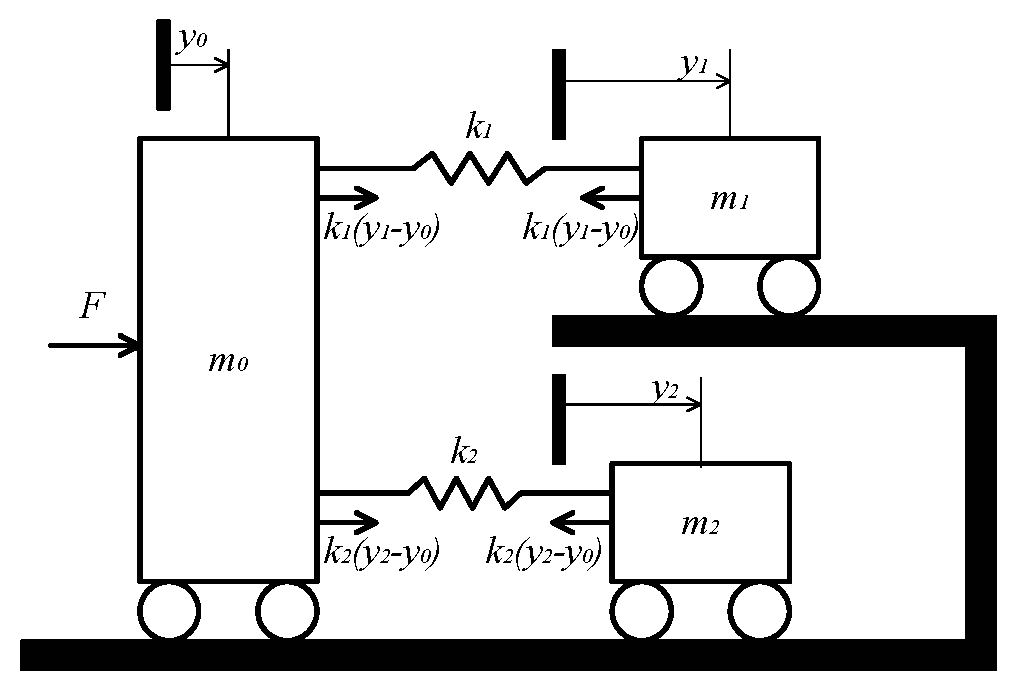
\epsfig{file=car3.eps,scale=0.7}
 \end{center}
\end{figure}

\newpage

\noindent
{\bf ３質量系}

次の３質量系の状態方程式を求めよ．
\begin{figure}[htbp]
 \begin{center}
　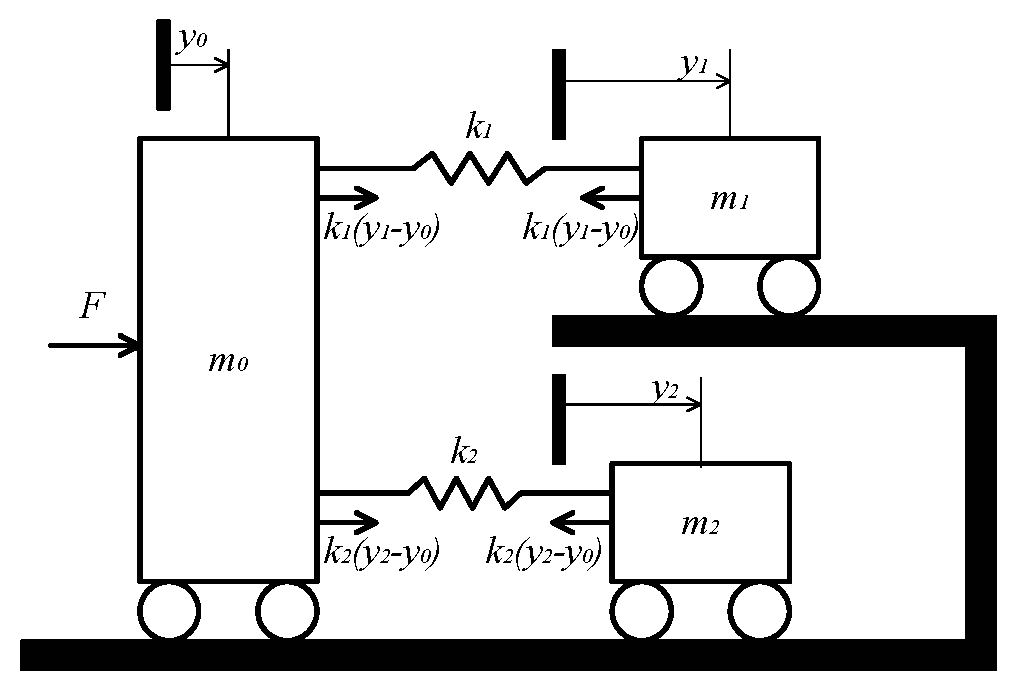
\epsfig{file=car3.eps,scale=0.7}
 \end{center}
\end{figure}
\begin{align}
	m_0 \ddot{y}_0 & = F + k_1 (y_1 - y_0) + k_2 (y_2-y_0)
\nonumber \\
	m_1 \ddot{y}_1 & = - k_1 (y_1 - y_0)
\nonumber \\
	m_2 \ddot{y}_2 & = - k_2 (y_2 - y_0)
\nonumber
\end{align}

\newpage

\noindent
{\bf ３質量系}

次の３質量系の状態方程式を求めよ．
\begin{figure}[htbp]
 \begin{center}
　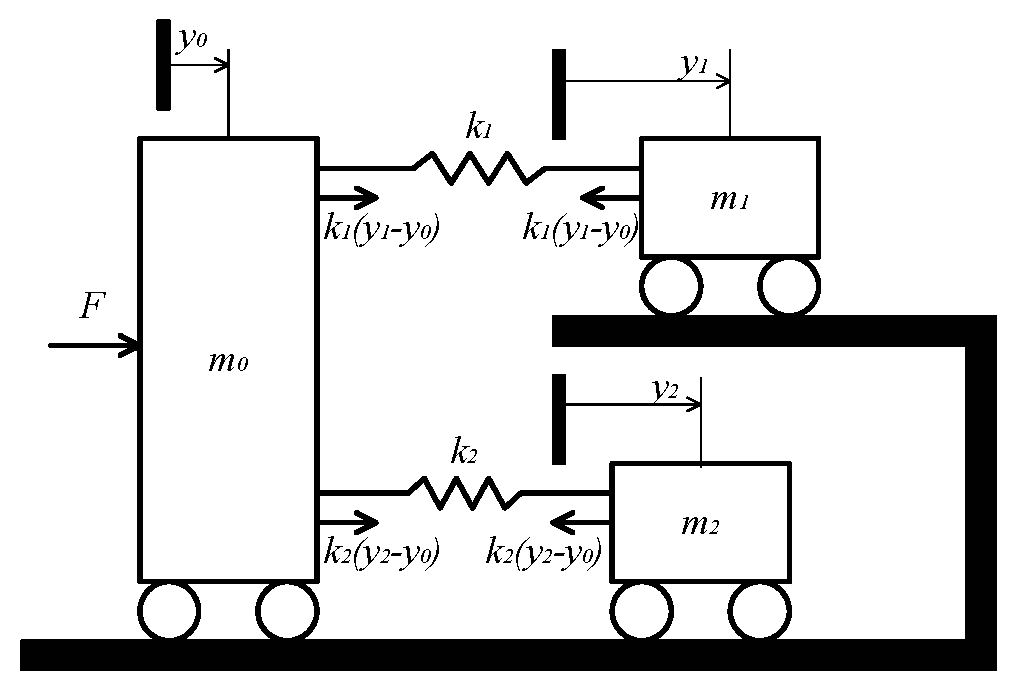
\epsfig{file=car3.eps,scale=0.7}
 \end{center}
\end{figure}
\begin{align}
	m_0 \ddot{y}_0 & = F + k_1 (y_1 - y_0) + k_2 (y_2-y_0)
\nonumber \\
	m_1 \ddot{y}_1 & = - k_1 (y_1 - y_0)
\nonumber \\
	m_2 \ddot{y}_2 & = - k_2 (y_2 - y_0)
\nonumber
\end{align}
よって状態方程式は
\begin{align}
 \frac{d}{dt} \left(\begin{array}{c}
	         y_0 \\
		     y_1 \\
		     y_2 \\
		     \frac{dy_0}{dt} \\
		     \frac{dy_1}{dt} \\
		     \frac{dy_2}{dt}
		    \end{array}\right)
 &=
 \left(\begin{array}{cccccc}
        0 & 0 & 0 & 1 & 0 & 0      \\
        0 & 0 & 0 & 0 & 1 & 0      \\
        0 & 0 & 0 & 0 & 0 & 1      \\
	-\frac{k_1}{m_0} -\frac{k_2}{m_0}&  \frac{k_1}{m_0} &  \frac{k_2}{m_0} & 0 & 0 & 0 \\
	 \frac{k_1}{m_1}                & -\frac{k_1}{m_1} &  0               & 0 & 0 & 0 \\
	 \frac{k_2}{m_2}                &  0               & -\frac{k_2}{m_2} & 0 & 0 & 0 
       \end{array}\right)
 \left(\begin{array}{c}
	         y_0 \\
		     y_1 \\
		     y_2 \\
		     \frac{dy_0}{dt} \\
		     \frac{dy_1}{dt} \\
		     \frac{dy_2}{dt}
       \end{array}\right)
 +
 \left(\begin{array}{c}
        0 \\
        0 \\
        0 \\
	    \frac{1}{m_0} \\
	    0 \\
	    0 
       \end{array}\right)
        F
\nonumber
\\
 \left(\begin{array}{c}
	    y_0 \\
		y_1 \\
		y_2
       \end{array}\right)
 &=
 \left(\begin{array}{cccccc}
         1 & 0 & 0 & 0 & 0 & 0  \\
         0 & 1 & 0 & 0 & 0 & 0 \\
         0 & 0 & 1 & 0 & 0 & 0 \\
       \end{array}\right)
 \left(\begin{array}{c}
	         y_0 \\
		     y_1 \\
		     y_2 \\
		     \frac{dy_0}{dt} \\
		     \frac{dy_1}{dt} \\
		     \frac{dy_2}{dt}
       \end{array}\right)
\nonumber
\end{align}


\newpage

\noindent
{\bf 可制御性の例題}

演習で用いた３質量系の状態方程式は
\begin{align}
 \frac{d}{dt} \left(\begin{array}{c}
	         y_0 \\
		     y_1 \\
		     y_2 \\
		     \frac{dy_0}{dt} \\
		     \frac{dy_1}{dt} \\
		     \frac{dy_2}{dt}
		    \end{array}\right)
 &=
 \left(\begin{array}{cccccc}
        0 & 0 & 0 & 1 & 0 & 0      \\
        0 & 0 & 0 & 0 & 1 & 0      \\
        0 & 0 & 0 & 0 & 0 & 1      \\
	-\frac{k_1}{m_0} -\frac{k_2}{m_0}&  \frac{k_1}{m_0} &  \frac{k_2}{m_0} & 0 & 0 & 0 \\
	 \frac{k_1}{m_1}                & -\frac{k_1}{m_1} &  0               & 0 & 0 & 0 \\
	 \frac{k_2}{m_2}                &  0               & -\frac{k_2}{m_2} & 0 & 0 & 0 
       \end{array}\right)
 \left(\begin{array}{c}
	         y_0 \\
		     y_1 \\
		     y_2 \\
		     \frac{dy_0}{dt} \\
		     \frac{dy_1}{dt} \\
		     \frac{dy_2}{dt}
       \end{array}\right)
 +
 \left(\begin{array}{c}
        0 \\
        0 \\
        0 \\
	    \frac{1}{m_0} \\
	    0 \\
	    0 
       \end{array}\right)
        F
\nonumber
\\
 \left(\begin{array}{c}
	    y_0 \\
		y_1 \\
		y_2
       \end{array}\right)
 &=
 \left(\begin{array}{cccccc}
         1 & 0 & 0 & 0 & 0 & 0  \\
         0 & 1 & 0 & 0 & 0 & 0 \\
         0 & 0 & 1 & 0 & 0 & 0 \\
       \end{array}\right)
 \left(\begin{array}{c}
	         y_0 \\
		     y_1 \\
		     y_2 \\
		     \frac{dy_0}{dt} \\
		     \frac{dy_1}{dt} \\
		     \frac{dy_2}{dt}
       \end{array}\right)
\nonumber
\end{align}
となる．このシステムについて以下を確認せよ．
\begin{itemize}
\item $m_0=m_1=m_2=1$, $k_1=k_2=1$のとき，システムは不可制御
\item $m_0=m_1=m_2=1$, $k_1=1$, $k_2=2$のとき，システムは可制御
\end{itemize}
$m_1=m_2$かつ$k_1=k_2$の場合には入力の直接作用する$m_0$に対して$m_1$と$m_2$は完全に同等のダイナミクスを持つため，独立に制御できなくなる．そのため不可制御となる．同様に$k_1/m_1 = k_2/m_2$の場合も不可制御となるが，それ以外の場合は可制御となる．

\newpage

\noindent
{\bf 可制御性の例題}
\begin{itemize}
\item $m_0=m_1=m_2=1$, $k_1=k_2=1$のとき
\end{itemize}

\begin{align}
 \frac{d}{dt} \left(\begin{array}{c}
	         y_0 \\
		     y_1 \\
		     y_2 \\
		     \frac{dy_0}{dt} \\
		     \frac{dy_1}{dt} \\
		     \frac{dy_2}{dt}
		    \end{array}\right)
 &=
 \left(\begin{array}{rrrrrr}
        0 & 0 & 0 & 1 & 0 & 0      \\
        0 & 0 & 0 & 0 & 1 & 0      \\
        0 & 0 & 0 & 0 & 0 & 1      \\
	-2& 1 & 1 & 0 & 0 & 0 \\
	1 & -1& 0 & 0 & 0 & 0 \\
	1 & 0 & -1& 0 & 0 & 0 
       \end{array}\right)
 \left(\begin{array}{c}
	         y_0 \\
		     y_1 \\
		     y_2 \\
		     \frac{dy_0}{dt} \\
		     \frac{dy_1}{dt} \\
		     \frac{dy_2}{dt}
       \end{array}\right)
 +
 \left(\begin{array}{c}
        0 \\
        0 \\
        0 \\
	    1 \\
	    0 \\
	    0 
       \end{array}\right)
        F
\nonumber
\\
 \left(\begin{array}{c}
	    y_0 \\
		y_1 \\
		y_2
       \end{array}\right)
 &=
 \left(\begin{array}{rrrrrr}
         1 & 0 & 0 & 0 & 0 & 0  \\
         0 & 1 & 0 & 0 & 0 & 0 \\
         0 & 0 & 1 & 0 & 0 & 0 \\
       \end{array}\right)
 \left(\begin{array}{c}
	         y_0 \\
		     y_1 \\
		     y_2 \\
		     \frac{dy_0}{dt} \\
		     \frac{dy_1}{dt} \\
		     \frac{dy_2}{dt}
       \end{array}\right)
\nonumber
\end{align}

可制御性のチェック

\begin{align}
 (B,AB, A^2B, A^3B, A^4B, A^5B)
 &=
 (B,AB, A(AB), A(A^2B), A(A^3B), A(A^4B))
\nonumber \\
 &=
 \left(\begin{array}{rrrrrr}
        0 & 1 & 0 & -2& 0 & 6      \\
        0 & 0 & 0 & 1 & 0 & -3      \\
        0 & 0 & 0 & 1 & 0 & -3      \\
	1 & 0 & -2& 0 & 6 & 0 \\
	0 & 0 & 1 & 0 & -3& 0 \\
	0 & 0 & 1 & 0 & -3& 0 
       \end{array}\right)
\nonumber
\end{align}
不可制御

\newpage

\noindent
{\bf 可制御性の例題}

\begin{itemize}
\item $m_0=m_1=m_2=1$, $k_1=1$, $k_2=2$のとき
\end{itemize}

\begin{align}
 \frac{d}{dt} \left(\begin{array}{c}
	         y_0 \\
		     y_1 \\
		     y_2 \\
		     \frac{dy_0}{dt} \\
		     \frac{dy_1}{dt} \\
		     \frac{dy_2}{dt}
		    \end{array}\right)
 &=
 \left(\begin{array}{rrrrrr}
        0 & 0 & 0 & 1 & 0 & 0      \\
        0 & 0 & 0 & 0 & 1 & 0      \\
        0 & 0 & 0 & 0 & 0 & 1      \\
	-3& 1 & 2 & 0 & 0 & 0 \\
	1 & -1& 0 & 0 & 0 & 0 \\
	2 & 0 & -2& 0 & 0 & 0 
       \end{array}\right)
 \left(\begin{array}{c}
	         y_0 \\
		     y_1 \\
		     y_2 \\
		     \frac{dy_0}{dt} \\
		     \frac{dy_1}{dt} \\
		     \frac{dy_2}{dt}
       \end{array}\right)
 +
 \left(\begin{array}{c}
        0 \\
        0 \\
        0 \\
	    1 \\
	    0 \\
	    0 
       \end{array}\right)
        F
\nonumber
\\
 \left(\begin{array}{c}
	    y_0 \\
		y_1 \\
		y_2
       \end{array}\right)
 &=
 \left(\begin{array}{rrrrrr}
         1 & 0 & 0 & 0 & 0 & 0  \\
         0 & 1 & 0 & 0 & 0 & 0 \\
         0 & 0 & 1 & 0 & 0 & 0 \\
       \end{array}\right)
 \left(\begin{array}{c}
	         y_0 \\
		     y_1 \\
		     y_2 \\
		     \frac{dy_0}{dt} \\
		     \frac{dy_1}{dt} \\
		     \frac{dy_2}{dt}
       \end{array}\right)
\nonumber
\end{align}

可制御性のチェック

\begin{align}
 (B,AB, A^2B, A^3B, A^4B, A^5B)
 &=
 (B,AB, A(AB), A(A^2B), A(A^3B), A(A^4B))
\nonumber \\
 &=
 \left(\begin{array}{rrrrrr}
        0 & 1 & 0 & -3& 0 & 14      \\
        0 & 0 & 0 & 1 & 0 & -4      \\
        0 & 0 & 0 & 2 & 0 &-10      \\
	1 & 0 & -3& 0 & 14& 0 \\
	0 & 0 & 1 & 0 & -4& 0 \\
	0 & 0 & 2 & 0 &-10& 0 
       \end{array}\right)
\nonumber
\end{align}
可制御

%---------------------------------------------------------------------------
\newpage

\noindent
{\bf 可観測性の例題}

演習の３質量系で，出力が$y=y0$の場合を考えると，状態方程式と出力方程式は
\begin{align}
 \frac{d}{dt} \left(\begin{array}{c}
	         y_0 \\
		     y_1 \\
		     y_2 \\
		     \frac{dy_0}{dt} \\
		     \frac{dy_1}{dt} \\
		     \frac{dy_2}{dt}
		    \end{array}\right)
 &=
 \left(\begin{array}{cccccc}
        0 & 0 & 0 & 1 & 0 & 0      \\
        0 & 0 & 0 & 0 & 1 & 0      \\
        0 & 0 & 0 & 0 & 0 & 1      \\
	-\frac{k_1}{m_0} -\frac{k_2}{m_0}&  \frac{k_1}{m_0} &  \frac{k_2}{m_0} & 0 & 0 & 0 \\
	 \frac{k_1}{m_1}                & -\frac{k_1}{m_1} &  0               & 0 & 0 & 0 \\
	 \frac{k_2}{m_2}                &  0               & -\frac{k_2}{m_2} & 0 & 0 & 0 
       \end{array}\right)
 \left(\begin{array}{c}
	         y_0 \\
		     y_1 \\
		     y_2 \\
		     \frac{dy_0}{dt} \\
		     \frac{dy_1}{dt} \\
		     \frac{dy_2}{dt}
       \end{array}\right)
 +
 \left(\begin{array}{c}
        0 \\
        0 \\
        0 \\
	    \frac{1}{m_0} \\
	    0 \\
	    0 
       \end{array}\right)
        F
\nonumber
\\
y &=
 \left(\begin{array}{cccccc}
         1 & 0 & 0 & 0 & 0 & 0
       \end{array}\right)
 \left(\begin{array}{c}
	         y_0 \\
		     y_1 \\
		     y_2 \\
		     \frac{dy_0}{dt} \\
		     \frac{dy_1}{dt} \\
		     \frac{dy_2}{dt}
       \end{array}\right)
\nonumber
\end{align}
となる．このシステムについて以下を確認せよ．
\begin{itemize}
\item $m_0=m_1=m_2=1$, $k_1=k_2=1$のとき，システムは不可観測
\item $m_0=m_1=m_2=1$, $k_1=1$, $k_2=2$のとき，システムは可観測
\end{itemize}
$m_1=m_2$かつ$k_1=k_2$の場合には出力$y_0$となる質量$m_0$に対して$m_1$と$m_2$は完全に同等のダイナミクスを持つため，両者の動きを区別することができなくなる．そのため不可観測となる．同様に$k_1/m_1 = k_2/m_2$の場合も不可観測となるが，それ以外の場合は可観測となる．

\newpage

\noindent
{\bf 可観測性の例題}

\begin{itemize}
\item $m_0=m_1=m_2=1$, $k_1=k_2=1$のとき
\end{itemize}
\begin{align}
 \frac{d}{dt} \left(\begin{array}{c}
	         y_0 \\
		     y_1 \\
		     y_2 \\
		     \frac{dy_0}{dt} \\
		     \frac{dy_1}{dt} \\
		     \frac{dy_2}{dt}
		    \end{array}\right)
 &=
 \left(\begin{array}{rrrrrr}
        0 & 0 & 0 & 1 & 0 & 0      \\
        0 & 0 & 0 & 0 & 1 & 0      \\
        0 & 0 & 0 & 0 & 0 & 1      \\
	-2& 1 & 1 & 0 & 0 & 0 \\
	1 & -1& 0 & 0 & 0 & 0 \\
	1 & 0 & -1& 0 & 0 & 0 
       \end{array}\right)
 \left(\begin{array}{c}
	         y_0 \\
		     y_1 \\
		     y_2 \\
		     \frac{dy_0}{dt} \\
		     \frac{dy_1}{dt} \\
		     \frac{dy_2}{dt}
       \end{array}\right)
 +
 \left(\begin{array}{c}
        0 \\
        0 \\
        0 \\
	    1 \\
	    0 \\
	    0 
       \end{array}\right)
        F
\nonumber
\\
y &=
 \left(\begin{array}{cccccc}
         1 & 0 & 0 & 0 & 0 & 0
       \end{array}\right)
 \left(\begin{array}{c}
	         y_0 \\
		     y_1 \\
		     y_2 \\
		     \frac{dy_0}{dt} \\
		     \frac{dy_1}{dt} \\
		     \frac{dy_2}{dt}
       \end{array}\right)
\nonumber
\end{align}

可観測性のチェック

\begin{align}
 \left(\begin{array}{l}
        C \\
        CA \\
        CA^2  \\
	CA^3 \\
	CA^4 \\
	CA^5
       \end{array}\right)
 &=
 \left(\begin{array}{l}
        C \\
        CA \\
        (CA)A  \\
	(CA^2)A \\
	(CA^3)A \\
	(CA^4)A
       \end{array}\right)
 =
 \left(\begin{array}{rrrrrr}
        1 & 0 & 0 & 0 & 0 & 0      \\
        0 & 0 & 0 & 1 & 0 & 0      \\
        -2& 1 & 1 & 0 & 0 & 0      \\
	0 & 0 & 0 & -2& 1 & 1 \\
	6 & -3& -3& 0 & 0 & 0 \\
	0 & 0 & 0 & 6 & -3& -3 
       \end{array}\right)
\nonumber
\end{align}
不可観測




\newpage

\noindent
{\bf 可観測性の例題}

\begin{itemize}
\item $m_0=m_1=m_2=1$, $k_1=1$, $k_2=2$のとき
\end{itemize}

\begin{align}
 \frac{d}{dt} \left(\begin{array}{c}
	         y_0 \\
		     y_1 \\
		     y_2 \\
		     \frac{dy_0}{dt} \\
		     \frac{dy_1}{dt} \\
		     \frac{dy_2}{dt}
		    \end{array}\right)
 &=
 \left(\begin{array}{rrrrrr}
        0 & 0 & 0 & 1 & 0 & 0      \\
        0 & 0 & 0 & 0 & 1 & 0      \\
        0 & 0 & 0 & 0 & 0 & 1      \\
	-3& 1 & 2 & 0 & 0 & 0 \\
	1 & -1& 0 & 0 & 0 & 0 \\
	2 & 0 & -2& 0 & 0 & 0 
       \end{array}\right)
 \left(\begin{array}{c}
	         y_0 \\
		     y_1 \\
		     y_2 \\
		     \frac{dy_0}{dt} \\
		     \frac{dy_1}{dt} \\
		     \frac{dy_2}{dt}
       \end{array}\right)
 +
 \left(\begin{array}{c}
        0 \\
        0 \\
        0 \\
	    \frac{1}{m_0} \\
	    0 \\
	    0 
       \end{array}\right)
        F
\nonumber
\\
y &=
 \left(\begin{array}{cccccc}
         1 & 0 & 0 & 0 & 0 & 0
       \end{array}\right)
 \left(\begin{array}{c}
	         y_0 \\
		     y_1 \\
		     y_2 \\
		     \frac{dy_0}{dt} \\
		     \frac{dy_1}{dt} \\
		     \frac{dy_2}{dt}
       \end{array}\right)
\nonumber
\end{align}

可観測性のチェック

\begin{align}
 \left(\begin{array}{l}
        C \\
        CA \\
        CA^2  \\
	CA^3 \\
	CA^4 \\
	CA^5
       \end{array}\right)
 &=
 \left(\begin{array}{l}
        C \\
        CA \\
        (CA)A  \\
	(CA^2)A \\
	(CA^3)A \\
	(CA^4)A
       \end{array}\right)
 =
 \left(\begin{array}{rrrrrr}
        1 & 0 & 0 & 0 & 0 & 0      \\
        0 & 0 & 0 & 1 & 0 & 0      \\
        -3& 1 & 2 & 0 & 0 & 0      \\
	0 & 0 & 0 & -3& 1 & 2 \\
	14& -4&-10& 0 & 0 & 0 \\
	0 & 0 & 0 & 14& -4&-10
       \end{array}\right)
\nonumber
\end{align}
可観測
%---------------------------------------------------------------------------
\newpage
\noindent
{\bf 電気回路　$RC$回路}

電気回路は$C$の電圧，$L$の電流を状態とすると状態方程式が求められる．
\begin{figure}[htbp]
 \begin{center}
　\epsfig{file=RC.eps,scale=1.5}
 \end{center}
\end{figure}

回路の基本方程式
\begin{align*}
	v_R &= i R \\
	i & = C \frac{d v_C}{dt} \\
	v_i & = v_R + v_C \\
	v_o & = v_C
\end{align*}
状態を$v_C$とするとその微分が必要だから
\begin{align*}
	\frac{d v_C}{dt} 
	&= \frac{i}{C} 
	= \frac{v_R/R}{C} 
	= \frac{v_R}{RC} 
	= \frac{v_i - v_C}{RC} 
	= - \frac{1}{RC} v_C + \frac{1}{RC} v_i \\
	v_o & = v_C
\end{align*}
%---------------------------------------------------------------------------
\newpage

\noindent
{\bf 電気回路　$LR$回路}

電気回路は$C$の電圧，$L$の電流を状態とすると状態方程式が求められる．
\begin{figure}[htbp]
 \begin{center}
　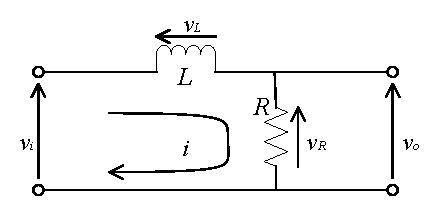
\epsfig{file=LR.eps,scale=1.5}
 \end{center}
\end{figure}

回路の基本方程式
\begin{align*}
	v_L & = L \frac{d i}{dt} \\
	v_R &= i R \\
	v_i & = v_L + v_R \\
	v_o & = v_R
\end{align*}
状態を$i$とするとその微分が必要だから
\begin{align*}
	\frac{d i}{dt} 
	&= \frac{v_L}{L} 
	= \frac{v_i - v_R}{L} 
	= - \frac{1}{L} v_R + \frac{1}{L} v_i 
	= - \frac{1}{L} R i + \frac{1}{L} v_i 
	= - \frac{R}{L} i + \frac{1}{L} v_i \\
	v_o & = v_R = R i
\end{align*}


%---------------------------------------------------------------------------
\newpage
\noindent
{\bf 電気回路　$LCR$回路}

電気回路は$C$の電圧，$L$の電流を状態とすると状態方程式が求められる．
\begin{figure}[htbp]
 \begin{center}
　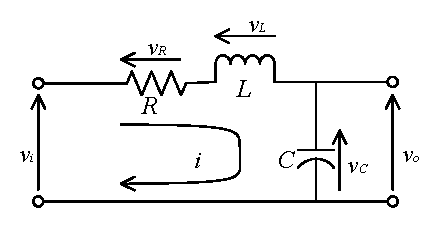
\epsfig{file=LCR.eps,scale=1.5}
 \end{center}
\end{figure}


%---------------------------------------------------------------------------
\newpage
\noindent
{\bf 電気回路　$LCR$回路}

電気回路は$C$の電圧，$L$の電流を状態とすると状態方程式が求められる．
\begin{figure}[htbp]
 \begin{center}
　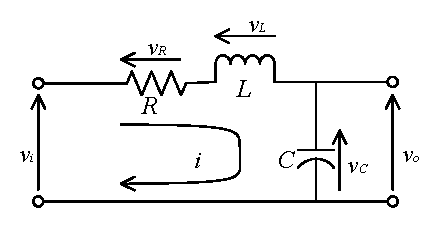
\epsfig{file=LCR.eps,scale=1.5}
 \end{center}
\end{figure}

回路の基本方程式
\begin{align*}
	v_L & = L \frac{d i}{dt} \\
	i & = C \frac{d v_C}{dt} \\
	v_R &= i R \\
	v_i & = v_L + v_C + v_R \\
	v_o & = v_C
\end{align*}

%---------------------------------------------------------------------------
\newpage
\noindent
{\bf 電気回路　$LCR$回路}

電気回路は$C$の電圧，$L$の電流を状態とすると状態方程式が求められる．
\begin{figure}[htbp]
 \begin{center}
　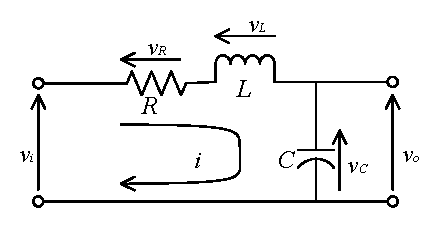
\epsfig{file=LCR.eps,scale=1.5}
 \end{center}
\end{figure}

回路の基本方程式
\begin{align*}
	v_L & = L \frac{d i}{dt} \\
	i & = C \frac{d v_C}{dt} \\
	v_R &= i R \\
	v_i & = v_L + v_C + v_R \\
	v_o & = v_C
\end{align*}
状態を$i$, $v_C$とするとその微分が必要だから
\begin{align*}
	\frac{d i}{dt} 
	&= \frac{v_L}{L} 
	= \frac{v_i - v_C - v_R}{L} 
	= - \frac{1}{L} v_R - \frac{1}{L} v_C + \frac{1}{L} v_i 
\\ &
	= - \frac{1}{L} R i - \frac{1}{L} v_C + \frac{1}{L} v_i 
	= - \frac{R}{L} i - \frac{1}{L} v_C + \frac{1}{L} v_i \\
	\frac{d v_C}{dt}
	&= \frac{i}{C} 
	= \frac{1}{C} i \\
	v_o &= v_C 
\end{align*}
よって状態方程式は
\begin{align*}
	\frac{d}{dt}
	\left (
	\begin{array}{c}
		i \\
		v_C
	\end{array}
	\right )
	&=
	\left (
	\begin{array}{cc}
		-\frac{R}{L} & -\frac{1}{L} \\
		\frac{i}{C} & 0 \\
	\end{array}
	\right )
	\left (
	\begin{array}{c}
		i \\
		v_C
	\end{array}
	\right )
	+
	\left (
	\begin{array}{c}
		\frac{1}{L} \\
		0
	\end{array}
	\right )
	v_i
\\
	v_o 
	&=
	\left (
	\begin{array}{cc}
		0 & 1 
	\end{array}
	\right )
	\left (
	\begin{array}{c}
		i \\
		v_C
	\end{array}
	\right )
\end{align*}


%---------------------------------------------------------------------------
\newpage

\noindent
{\bf 不可制御なシステムの分解（演習）}

次のシステムが不可制御であることを確認し，可制御な部分と不可制御な部分に分けよ．\begin{align*}
	\frac{d}{dt}
	\left (
	\begin{array}{c}
	 x_1 \\ x_2 
	\end{array}
	\right )
	& = 
	\left (
	\begin{array}{cc}
	 0 & 1 \\
	 -1 & 2
	\end{array}
	\right )
	\left (
	\begin{array}{c}
	 x_1 \\ x_2 
	\end{array}
	\right )
	+
	\left (
	\begin{array}{c}
	 1 \\ 1 
	\end{array}
	\right )
	u
\\
	y 
	&=
	\left (
	\begin{array}{cc}
	 1 & 1  
	\end{array}
	\right )
	\left (
	\begin{array}{c}
	 x_1 \\ x_2 
	\end{array}
	\right )
\end{align*}

%---------------------------------------------------------------------------
\newpage

\noindent
{\bf 不可制御なシステムの分解（演習）}

次のシステムが不可制御であることを確認し，可制御な部分と不可制御な部分に分けよ．\begin{align*}
	\frac{d}{dt}
	\left (
	\begin{array}{c}
	 x_1 \\ x_2 
	\end{array}
	\right )
	& = 
	\left (
	\begin{array}{cc}
	 0 & 1 \\
	 -1 & 2
	\end{array}
	\right )
	\left (
	\begin{array}{c}
	 x_1 \\ x_2 
	\end{array}
	\right )
	+
	\left (
	\begin{array}{c}
	 1 \\ 1 
	\end{array}
	\right )
	u
\\
	y 
	&=
	\left (
	\begin{array}{cc}
	 1 & 1  
	\end{array}
	\right )
	\left (
	\begin{array}{c}
	 x_1 \\ x_2 
	\end{array}
	\right )
\end{align*}

\begin{align*}
	(B, AB) 
	& =
	\left (
	\begin{array}{cc}
	 1 & 1\\ 
	 1 & 1
	\end{array}
	\right )
\\
	T
	&=
	\left (
	\begin{array}{cc}
	 1 & 0\\ 
	 1 & 1
	\end{array}
	\right )
\\
	T^{-1}
	&=
	\left (
	\begin{array}{cc}
	 1 & 0\\ 
	 -1 & 1
	\end{array}
	\right )
\\
	\bar{A} 
	&= 
	T^{-1} A T
	=
	\left (
	\begin{array}{cc}
	 1 & 0\\ 
	 -1 & 1
	\end{array}
	\right )
	\left (
	\begin{array}{cc}
	 0 & 1 \\
	 -1 & 2
	\end{array}
	\right )
	\left (
	\begin{array}{cc}
	 1 & 0\\ 
	 1 & 1
	\end{array}
	\right )
\\	
	&	\hspace*{2cm}
	=
	\left (
	\begin{array}{cc}
	 0 & 1 \\
	 -1 & 1
	\end{array}
	\right )
	\left (
	\begin{array}{cc}
	 1 & 0\\ 
	 1 & 1
	\end{array}
	\right )
	=
	\left (
	\begin{array}{cc}
	 1 & 1\\ 
	 0 & 1
	\end{array}
	\right )
\\
	\bar{B}
	&=
	T^{-1}B
	=
	\left (
	\begin{array}{cc}
	 1 & 0\\ 
	 -1 & 1
	\end{array}
	\right )
	\left (
	\begin{array}{c}
	 1 \\ 1 
	\end{array}
	\right )
	=
	\left (
	\begin{array}{c}
	 1 \\ 0
	\end{array}
	\right )
\\
	\bar{C}
	&=
	C T
	=
	\left (
	\begin{array}{cc}
	 1 & 1  
	\end{array}
	\right )
	\left (
	\begin{array}{cc}
	 1 & 0\\ 
	 1 & 1
	\end{array}
	\right )
	=
	\left (
	\begin{array}{cc}
	 2 & 1  
	\end{array}
	\right )
\end{align*}


%---------------------------------------------------------------------------
\newpage

\noindent
{\bf 極配置（演習）}

次の状態方程式
\begin{align*}
	\frac{d}{dt}
	\left (
	\begin{array}{c}
	 x_1 \\ x_2 
	\end{array}
	\right )
	& = 
	\left (
	\begin{array}{cc}
	 0 & 1 \\
	 0 & -1
	\end{array}
	\right )
	\left (
	\begin{array}{c}
	 x_1 \\ x_2 
	\end{array}
	\right )
	+
	\left (
	\begin{array}{c}
	 0 \\ 1 
	\end{array}
	\right )
	u
\end{align*}
に対して閉ループ系の極が$-4,-5$となるような状態フィードバック
\begin{align*}
	u 
	&=
	\left (
	\begin{array}{cc}
	 f_1 & f_2
	\end{array}
	\right )
	\left (
	\begin{array}{c}
	 x_1 \\ x_2 
	\end{array}
	\right )
\end{align*}
を求めよ．

%---------------------------------------------------------------------------
\newpage

\noindent
{\bf 極配置（演習）}

次の状態方程式
\begin{align*}
	\frac{d}{dt}
	\left (
	\begin{array}{c}
	 x_1 \\ x_2 
	\end{array}
	\right )
	& = 
	\left (
	\begin{array}{cc}
	 0 & 1 \\
	 0 & -1
	\end{array}
	\right )
	\left (
	\begin{array}{c}
	 x_1 \\ x_2 
	\end{array}
	\right )
	+
	\left (
	\begin{array}{c}
	 0 \\ 1 
	\end{array}
	\right )
	u
\end{align*}
に対して閉ループ系の極が$-4,-5$となるような状態フィードバック
\begin{align*}
	u 
	&=
	\left (
	\begin{array}{cc}
	 f_1 & f_2
	\end{array}
	\right )
	\left (
	\begin{array}{c}
	 x_1 \\ x_2 
	\end{array}
	\right )
\end{align*}
を求めよ．
\\

閉ループ系は
\begin{align*}
	\frac{d}{dt}
	\left (
	\begin{array}{c}
	 x_1 \\ x_2 
	\end{array}
	\right )
	& = 
	\left (
	\begin{array}{cc}
	 0 & 1 \\
	 0 & -1
	\end{array}
	\right )
	\left (
	\begin{array}{c}
	 x_1 \\ x_2 
	\end{array}
	\right )
	+
	\left (
	\begin{array}{c}
	 0 \\ 1 
	\end{array}
	\right )
	\left (
	\begin{array}{cc}
	 f_1 & f_2
	\end{array}
	\right )
	\left (
	\begin{array}{c}
	 x_1 \\ x_2 
	\end{array}
	\right )
\\
	&=
	\left (
	\begin{array}{cc}
	 0 & 1 \\
	 0 & -1
	\end{array}
	\right )
	\left (
	\begin{array}{c}
	 x_1 \\ x_2 
	\end{array}
	\right )
	+
	\left (
	\begin{array}{cc}
	 0   & 0   \\
	 f_1 & f_2
	\end{array}
	\right )
	\left (
	\begin{array}{c}
	 x_1 \\ x_2 
	\end{array}
	\right )
\\
	&=
	\left (
	\begin{array}{cc}
	 0 & 1 \\
	 f_1 & f_2-1
	\end{array}
	\right )
	\left (
	\begin{array}{c}
	 x_1 \\ x_2 
	\end{array}
	\right )
\end{align*}
特性多項式は
\begin{align*}
	\mbox{det}[sI-(A+BF)]
	& =
	\mbox{det}
	\left (
	\begin{array}{cc}
	 s & - 1 \\
	 - f_1 & s- (f_2-1)
	\end{array}
	\right )
\\
	&= s [s-(f_2-1)] - f_1
\\
	&= s^2 - (f_2-1) s - f_1
\end{align*}
望ましい特性多項式は望ましい極が$-4,-5$であることより
\begin{align*}
	(s+4)(s+5) = s^2 + 9s + 20
\end{align*}
よって係数を比較して
\begin{align*}
	-(f_2-1)=9, \ \ \ -f_1=20
\end{align*}
よって
\begin{align*}
	f_2=-8, \ \ \ f_1=-20
\end{align*}

%---------------------------------------------------------------------------
\newpage

\noindent
{\bf 最適制御（演習）}

次のシステムと評価関数に対する最適制御を求めよ．
\begin{align*}
	\frac{dx}{dt} & = 1 \cdot x + 1 \cdot u \ \ \ \ \ \ \ \ \ \ \ \ A=1,B=1\\
	J & = \int_0^{\infty} x^2 + r u^2 dt \ \ \ \ \ \ \ \ Q=1,R=r
\end{align*}


%---------------------------------------------------------------------------
\newpage

\noindent
{\bf 最適制御（演習）}

次のシステムと評価関数に対する最適制御を求めよ．
\begin{align*}
	\frac{dx}{dt} & = 1 \cdot x + 1 \cdot u \ \ \ \ \ \ \ \ \ \ \ \ A=1,B=1\\
	J & = \int_0^{\infty} x^2 + r u^2 dt \ \ \ \ \ \ \ \ Q=1,R=r
\end{align*}

Riccati方程式
\begin{align*}
	& A^T P + P A - P B R^{-1} B^T P + Q = 0 \\
	& 1 \cdot p + p \cdot 1 - p \cdot 1 \cdot \frac{1}{r} \cdot 1 \cdot p + 1 = 0 \\
	& \frac{-1}{r} p^2 + 2p + 1 = 0 \\
	& p^2 -2rp - r = 0
\end{align*}
よって
\begin{align*}
	p = r \pm \sqrt{r^2 + r}
\end{align*}
$p>0$より
\begin{align*}
	p = r + \sqrt{r^2+r}
\end{align*}
最適制御は
\begin{align*}
	u &= -R^{-1}B^T P x \\
	&= -\frac{1}{r} \cdot 1 \cdot (r + \sqrt{r^2+r}) x \\
	&= (-1 - \sqrt{1 + (1/r)}) x
\end{align*}
閉ループ系は
\begin{align*}
	\frac{dx}{dt} & = 1 \cdot x + 1 \cdot u \\
	&= 1 \cdot x + 1 \cdot (-1 - \sqrt{1 + (1/r)}) x \\
	&= - \sqrt{1 + (1/r)}) x
\end{align*}
となる．閉ループ系の極は
\begin{align*}
	\begin{array}{lccr}
		r \rightarrow 0 & : && - \infty \\
		r \rightarrow \infty & : && -1 \\
	\end{array}
\end{align*}
これは$R$を小さくすると入力$u$に対する重みが小さくなるので，入力をいっぱい使って速く状態を収束させる制御系が設計されることと一致する．

%---------------------------------------------------------------------------
\newpage

$M$と$M^T$の固有値が等しいことは以下のように証明できる．行列$M$に対し，
\begin{align}
   T^{-1}MT = \Lambda
\end{align}
と対角化できたとする．この時$\Lambda$の対角要素は$M$の固有値からなっている．ここで$T^{-1}MT$を
転置すると，
\begin{align}
   (T^{-1}MT)^T &=  \Lambda^T = \Lambda
\\
   (T^{-1}MT)^T &= T^T M^T T^{-T} = (T^{-T})^{-1} M^T T^{-T} = \bar{T}^{-1} M^T \bar{T}
   , \ \ \ \bar{T} = T^{-1}
\end{align}
より
\begin{align}
   \bar{T}^{-1} M^T \bar{T} &=  \Lambda
\end{align}
となる．これは$M^{T}$が$\bar{T}$により$\Lambda$に対角化されることを意味しているので，
$\Lambda$の対角要素は$M^{T}$の固有値でもある．つまり，$M$と$M^{T}$
の固有値は等しい．


\end{document}

%--------------------------------------------------------------------------------
\noindent
{\bf 可制御正準形}
%---------------------------------------------------------------------------



伝達関数
\begin{equation}
 G(s) =
  \frac{b_{n-1} s^{n-1} + b_{n-2} s^{n-2} + \cdots + b_1 s + b_0}
  {s^n + a_{n-1} s^{n-1} + a_{n-2} s^{n-2} + \cdots + a_1 s + a_0}
  + d
  \label{eq:G(s)}
\end{equation}
は以下の状態方程式で表される．このシステムは{\bf {可制御正準形}(controller canonical form)}と呼ばれる．
\begin{align}
 \frac{d}{dt}
  \left(\begin{array}{c}
         x_1 \\
	 x_2 \\
	 \vdots \\
	 x_{n-1} \\
	 x_n
	\end{array}\right)
  &=
  \left(\begin{array}{ccccc}
     0      & 1      & 0      & \cdots & 0 \\
	 0      & 0      & 1      & \ddots & \vdots \\
	 \vdots & \vdots & \ddots & \ddots & 0 \\
	 0      & 0      & \cdots & 0      & 1 \\
	 -a_0   & -a_1   & \cdots & -a_{n-2} & -a_{n-1}
	\end{array}\right)
  \left(\begin{array}{c}
	 x_1 \\
	 x_2 \\
	 \vdots \\
	 x_{n-1} \\
	 x_n
	\end{array}\right)
  +
  \left(\begin{array}{c}
         0 \\
	 0 \\
	 \vdots \\
	 0 \\
	 1
	\end{array}\right)
  u \label{eq:canoform}\\
y &=
 \left(\begin{array}{ccccc}
        b_0 & b_1 & \cdots & b_{n-2} & b_{n-1}
       \end{array}\right)
 \left(\begin{array}{c}
        x_1 \\
	x_2 \\
	\vdots \\
	x_{n-1} \\
	x_n
       \end{array}\right)
 + d u
\end{align}
これは以下のように証明できる．まず，
$(sI-A)^{-1}$が
